\documentclass[10pt]{extarticle}
\usepackage[a4paper,margin=1.6cm]{geometry}
\usepackage{amsmath,amssymb,bm,enumitem,titlesec,xcolor,booktabs,array,graphicx}
\titleformat{\section}{\large\bfseries\color{blue!50!black}}{\thesection.}{0.5em}{}
\titlespacing*{\section}{0pt}{8pt}{3pt}
\titleformat{\subsection}{\normalsize\bfseries}{}{0em}{}
\titlespacing*{\subsection}{0pt}{5pt}{2pt}
\setlist{nosep,leftmargin=1.3em}
\setlength{\parindent}{0pt}\setlength{\parskip}{4pt}
\newcommand{\B}{\mathbf B}\newcommand{\J}{\mathbf J}\newcommand{\F}{\mathbf F}\newcommand{\zh}{\hat{\mathbf z}}
\pagestyle{plain}
\begin{document}
{\Large\bfseries The Poisson pressure step: a fast magnetohydrostatic correction}\\[2pt]
{\small Physics of the \texttt{poisson-step} branch (\texttt{HSEMHS/scripts/poisson/poisson\_step.jl}). HSEMHS code, 23 Oct 2026.}

\section{Why a second method}
The joint solver (M5h) changes both the pressure $P$ and the magnetic field $\B$ until the forces balance. On the full
Bifrost cube ($504\times504\times496$) it needs more than 24\,h on four nodes. That is fine for one atmosphere, but not
inside a Stokes inversion, where the atmosphere changes at every iteration and the force balance has to be restored
each time.

The FIRTEZ-dz inversion code (Borrero et al.) solves this problem differently: it keeps $T$ and $\B$ as the inversion gives
them and corrects \emph{only the pressure}, by solving a Poisson equation. This branch implements that idea for our grid
and our equation of state, and measures what it can and cannot do.

\section{The quantities}
\renewcommand{\arraystretch}{1.15}
\begin{tabular}{>{$}l<{$} p{10.6cm} l}
\toprule
\text{Symbol} & Meaning & Unit \\ \midrule
x,\,y,\,z & horizontal coordinates (periodic box, $\Delta x=47.6$\,km) and height ($-2.44$ to $14.37$\,Mm) & m \\
T & temperature, from Bifrost snapshot 385, \textbf{fixed} & K \\
\B & magnetic field, from Bifrost, \textbf{fixed} in this method & T \\
\J & current density $\nabla\times\B/\mu_0$ & A\,m$^{-2}$ \\
P & gas pressure: the only unknown & Pa \\
u & $\ln P$, the variable actually solved for & -- \\
\rho & density, $\rho=\rho(T,P)$ from the EOS table \texttt{cache/eos\_table\_fullz.h5} (includes ionisation) & kg\,m$^{-3}$ \\
g & 274, gravity points along $-\zh$ & m\,s$^{-2}$ \\
H & pressure scale height $P/(\rho g)=k_BT/(\bar\mu m_{\rm H} g)$, about 100--150\,km in the photosphere & m \\
\beta & plasma beta, $2\mu_0P/B^2$: gas pressure over magnetic pressure & -- \\
\tau_{500} & optical depth at 500\,nm, integrated down from the top of the box & -- \\
z_{\rm cut} & top of the region where the force balance is solved (1\,Mm in production) & m \\
\bottomrule
\end{tabular}

\section{The equation to satisfy}
A static atmosphere needs zero net force per unit volume at every point:
\[
\F \;\equiv\; -\nabla P \;+\; \J\times\B \;-\; \rho g\,\zh \;=\; 0 .
\]
In this method $\J\times\B$ is a \emph{given} force field (computed once from the fixed $\B$), and $\rho g$ depends on $P$
only through the EOS. So the question is: \emph{which pressure field balances gravity plus a given Lorentz force?}

\textbf{Why it is called a Poisson step.} Take the divergence of $\F=0$:
\[
\nabla^2 P \;=\; \nabla\!\cdot(\J\times\B) \;-\; g\,\frac{\partial\rho}{\partial z}.
\]
This is a Poisson equation for $P$ (FIRTEZ solves essentially this, with the right-hand side evaluated from the current
atmosphere and iterated). A Poisson equation can be solved very quickly: in a periodic box the horizontal directions
separate into Fourier modes, and each mode is a one-dimensional problem in $z$.

\section{Gradient and non-gradient forces: what a pressure correction can and cannot do}

\subsection*{4.1 The decomposition}
Any force field $\F(x,y,z)$ in our box can be split uniquely into two parts (the \emph{Helmholtz decomposition}):
\[
\F \;=\; \underbrace{-\nabla\phi}_{\text{gradient part}} \;+\; \underbrace{\mathbf S}_{\text{non-gradient part}},
\qquad\text{with } \mathbf S \text{ ``orthogonal'' to every gradient: } \int \mathbf S\cdot\nabla\psi\;dV=0 \text{ for all } \psi .
\]
\begin{itemize}
\item The \textbf{gradient part} $-\nabla\phi$ is a force that can be written as the slope of a scalar ``potential''
$\phi$, just as a pressure force is the slope of $P$. It has no curl: $\nabla\times\nabla\phi=0$.
\item The \textbf{non-gradient part} $\mathbf S$ is everything else. It contains all of the curl of $\F$:
$\nabla\times\mathbf S=\nabla\times\F$. Orthogonality to all gradients means (integrating by parts, periodic in $x,y$)
$\nabla\cdot\mathbf S=0$ inside the box: $\mathbf S$ is a pure ``swirl''.
\item The two parts are orthogonal, so their sizes add like the sides of a right triangle:
$\int|\F|^2dV=\int|\nabla\phi|^2dV+\int|\mathbf S|^2dV$.
\end{itemize}
\textbf{Why this matters here.} Changing the pressure by $\delta P$ changes the force by $-\nabla\delta P$, a pure gradient.
If the density did not change, a pressure correction could therefore remove the gradient part exactly ($\delta P=-\phi$)
and could \emph{never} touch $\mathbf S$. $\int|\mathbf S|^2dV$ would be a hard floor for any pressure-only method.

\subsection*{4.2 Which forces are gradients?}
Write out the curl of the force balance. Using $\nabla\times\nabla P=0$ and $\nabla\times(\rho g\zh)=g(\partial_y\rho,\,-\partial_x\rho,\,0)$:
\[
\nabla\times\F \;=\; \nabla\times(\J\times\B) \;-\; g\left(\frac{\partial\rho}{\partial y},\;-\frac{\partial\rho}{\partial x},\;0\right) .
\]
Term by term:
\begin{enumerate}
\item \textbf{Pressure, $-\nabla P$:} always a gradient. This is the only term the Poisson step controls directly.
\item \textbf{Gravity, $-\rho g\zh$:} a gradient \emph{only if $\rho$ is the same everywhere on each horizontal plane}. Any
horizontal density contrast makes a non-gradient part. This is buoyancy: next to each other at the same height, a light
(hot) column and a heavy (cool) column cannot be in static balance, because the weight of the heavy column makes the pressure
below it increase faster with depth than below the light one, and the resulting sideways pressure push has nowhere to go.
\item \textbf{Lorentz force, $\J\times\B=-\nabla\!\left(B^2/2\mu_0\right)+(\B\cdot\nabla)\B/\mu_0$:} the magnetic
pressure is a gradient; the magnetic tension in general is not. Its curl, $\nabla\times(\J\times\B)$, is the only thing that can
hold up horizontal density contrasts.
\end{enumerate}
So static equilibrium requires
\[
\nabla\times(\J\times\B) \;=\; g\left(\frac{\partial\rho}{\partial y},\;-\frac{\partial\rho}{\partial x},\;0\right)
\qquad\text{(curl condition)} .
\]
\textbf{Without a magnetic field} this says $\partial_x\rho=\partial_y\rho=0$, and the horizontal force components then give
$\partial_xP=\partial_yP=0$: the only static non-magnetic atmosphere is horizontally uniform (each plane one $P$, one $\rho$).
Bifrost's granulation has hot upflows next to cool downflows, so with $T$ fixed and $\rho=\rho(T,P)$ this is impossible:
\emph{no choice of pressure makes a Bifrost temperature field exactly static without help from $\B$.} In the magnetic
case the tension of the fixed field would have to supply exactly the right curl at every point, which it will not, since
Bifrost's $\B$ was never shaped for that.

\subsection*{4.3 The density loophole}
The floor in 4.1 assumed that $\rho$ stays fixed. It does not: $\rho=\rho(T,P)$, and with $T$ fixed
\[
\delta\rho \;=\; \rho\,\frac{\partial\ln\rho}{\partial\ln P}\Big|_T\,\frac{\delta P}{P}
\qquad\Rightarrow\qquad
\delta(\nabla\times\F) \;=\; -g\,\nabla\times(\delta\rho\,\zh) .
\]
So a pressure change does alter the curl of $\F$, through the density and gravity. Making the pressure fall faster with
height under a dense column lowers its density at a given height, which shrinks the horizontal density contrast and the
non-gradient part. The Poisson step can therefore reduce $\mathbf S$ too, but only partly, and only by tuning the density
through $P$ (it cannot touch the part that comes from the temperature contrast at fixed pressure, or from the tension of $\B$).
The non-gradient part measured with $\rho$ held fixed is therefore \emph{not} a strict floor for the Poisson step. It is a
reference level, which the step can beat in some layers and not in others (4.5).

\subsection*{4.4 How the split is computed}
The diagnostic \texttt{scripts/m5\_bifrost/force\_split.py} does the decomposition on the same grid as the Poisson step:
\begin{itemize}
\item $P$, $\rho$, $\B$ at cell centres; $F_x,F_y$ at cell centres with centred periodic differences; $F_z$ on the faces
between layers, $F_z=-(P_{k+1}-P_k)/h-g(\rho_k+\rho_{k+1})/2+(L_{z,k}+L_{z,k+1})/2$ with $L=\J\times\B$.
\item ``Orthogonal'' is measured with layer weights: cell width divided by $S_k^2$, where $S_k$ is the median of $\rho g$
in layer $k$. Without the weights the deep, dense layers (where $\rho g$ is $10^{10}$ times larger than at the top) would
decide everything; with them, every layer counts in units of the weight of its own gas.
\item $\phi$ is found by solving the weighted normal equations $G^{\top}WG\,\phi=G^{\top}W\F$ ($G$ the discrete gradient):
FFT in $x,y$ and one tridiagonal solve in $z$ per Fourier mode, i.e.\ the same Poisson structure as the step itself.
Then $\mathbf S=\F+G\phi$.
\item Checks: on the full cube $\langle\mathbf S,G\phi\rangle/\|\F\|^2\approx10^{-16}$ and
$\|\F\|^2=\|G\phi\|^2+\|\mathbf S\|^2$ to $10^{-14}$. A synthetic pure-gradient field gives $\mathbf S=0$ exactly.
\item Orthogonality holds for the \emph{whole box}, not layer by layer. In one layer the two parts can partly cancel, so
the per-layer RMS values below need not satisfy $F^2=G^2+S^2$ exactly.
\end{itemize}

\subsection*{4.5 The measured split}
RMS over each layer, in units of the layer median of $\rho g$, for $|\F|$ / gradient part / non-gradient part:
\begin{center}\small
\begin{tabular}{r ccc ccc ccc ccc}
\toprule
& \multicolumn{3}{c}{Bifrost snapshot} & \multicolumn{3}{c}{column HSE (input)} & \multicolumn{3}{c}{\textbf{Poisson step}} & \multicolumn{3}{c}{M5h (iter.\ 132)}\\
\cmidrule(lr){2-4}\cmidrule(lr){5-7}\cmidrule(lr){8-10}\cmidrule(lr){11-13}
$z$ [Mm] & $|F|$ & grad & non & $|F|$ & grad & non & $|F|$ & grad & non & $|F|$ & grad & non \\ \midrule
$-1.0$  & .045 & .043 & .017 & .045 & .042 & .014 & .023 & .012 & .023 & .069 & .068 & .012 \\
$-0.5$  & .109 & .102 & .046 & .114 & .104 & .037 & .057 & .024 & .060 & .095 & .086 & .033 \\
$-0.25$ & .179 & .160 & .091 & .191 & .173 & .066 & .099 & .037 & .101 & .148 & .129 & .061 \\
$0.0$   & .295 & .251 & .114 & .330 & .264 & .136 & .127 & .053 & .099 & .268 & .196 & .127 \\
$0.25$  & .118 & .106 & .069 & .228 & .180 & .158 & .065 & .045 & .049 & .192 & .142 & .147 \\
$0.5$   & .121 & .102 & .072 & .220 & .170 & .144 & .063 & .038 & .053 & .179 & .126 & .131 \\
$0.75$  & .214 & .168 & .142 & .279 & .199 & .189 & .094 & .054 & .080 & .216 & .134 & .163 \\
$1.0$   & .488 & .363 & .362 & .664 & .467 & .418 & .336 & .266 & .205 & .509 & .362 & .342 \\
\bottomrule
\end{tabular}
\end{center}
What the table says:
\begin{enumerate}
\item \textbf{Column HSE is mostly a gradient error.} Each column is hydrostatic on its own, so what is missing is mainly
the horizontal pressure balance between columns, plus the magnetic pressure, both gradients. In the photosphere
($z\le0$) 80--90\,\% of $|\F|^2$ is gradient; at 0.25--1\,Mm about half.
\item \textbf{The Poisson step removes the gradient part.} It falls 3.5--5 times ($0.264\to0.053$ at $z=0$, $0.180\to0.045$ at
0.25\,Mm). What remains is now mostly non-gradient, as expected from a pressure-only correction.
\item \textbf{The non-gradient part changes too (density loophole, 4.3).} Between 0 and 0.75\,Mm it fell by a factor 1.4--3.2
($0.158\to0.049$ at 0.25\,Mm). Below $z=0$ it rose ($0.066\to0.101$ at $-0.25$\,Mm, $0.037\to0.060$ at $-0.5$\,Mm): the
step minimises $|\F|/P$ summed over all layers at once, and accepted a larger non-gradient part in the deep layers in
exchange for a much smaller total higher up. The total $|\F|$ still halved in every layer.
\item \textbf{Bifrost itself is not static.} Its imbalance is the inertia of the flows, $\rho\,D\mathbf v/Dt$. It too is
mostly gradient (pressure fluctuations of the convection), with a 15--35\,\% non-gradient share in the photosphere (buoyancy
of granules, which drives the convection).
\item \textbf{M5h at iteration 132} has a non-gradient part close to column HSE. It is measured here on a grid
that is not its own (M5h works on a staggered grid), so this column is only indicative.
\end{enumerate}
In short: a pressure-only method removes the gradient error almost completely and, through the density, part of the
non-gradient error. The rest, the buoyancy of the fixed temperature structure that the fixed field cannot hold up, can
only be removed by changing $\B$ (the joint solver) or $T$.

\section{Working in $u=\ln P$}
We divide the force by $P$ and solve for $u=\ln P$:
\[
\mathbf R \;\equiv\; \frac{\F}{P} \;=\; -\nabla u \;-\; \frac{\zh}{H(T,P)} \;+\; \frac{\J\times\B}{P}.
\]
Reasons:
\begin{enumerate}
\item \textbf{The pressure stays positive.} $P=e^u>0$ automatically, even across the 14 orders of magnitude in the box.
\item \textbf{No reward for collapsing the pressure.} Our first version minimised $|\F|^2$ itself. Because $\F$ scales
with $P$, the cheapest way to make $|\F|$ small is to make $P$ small: the solver drove $P$ towards zero in 637\,000 cells
and had to be clamped. $\mathbf R=\F/P$ is a \emph{relative} imbalance, so lowering $P$ no longer helps.
\item \textbf{Hydrostatic is natural.} Without the Lorentz force, $R_z=0$ is $du/dz=-1/H$: the familiar exponential
decrease of pressure with height.
\end{enumerate}
We minimise the weighted sum of squares
\[
\Phi(u) \;=\; \sum_{\text{cell centres}} w\,\bar H^2\,(R_x^2+R_y^2) \;+\; \sum_{z\text{-faces}} h\,\bar H^2\,R_z^2 ,
\]
where $w,h$ are the cell widths in $z$ and $\bar H$ is the layer median of $H$. Since $R\bar H\approx F/(\rho g)$, $\Phi$
measures the force imbalance \emph{in units of the weight of the gas}, layer by layer, so deep dense layers do not swamp
the upper ones. The discretisation is the cell-centred one also used by the diagnostic \texttt{force\_split.py}: $\B$ at
cell centres, centred periodic differences in $x,y$, $R_z$ on the faces between layers.

\section{How the minimum is found}
$\mathbf R$ depends on $u$ linearly through $-\nabla u$ and non-linearly through $\rho(T,P)$ in $1/H$ and through $1/P$ in
the Lorentz term. Each \textbf{Gauss--Newton} step linearises $\mathbf R(u+\delta u)\approx\mathbf R(u)+\mathbf J_R\,\delta u$
and solves the normal equations
\[
\mathbf J_R^{\!\top}W\mathbf J_R\;\delta u \;=\; -\mathbf J_R^{\!\top}W\mathbf R .
\]
The leading part of $\mathbf J_R^{\!\top}W\mathbf J_R$ is $-\nabla\!\cdot(W\nabla\,\cdot)$, a weighted Laplacian: \emph{each
step is a Poisson solve for $\delta u$}, plus local terms from the EOS and the Lorentz term. Numerically:
\begin{itemize}
\item \textbf{Conjugate gradients} on the normal equations, \textbf{preconditioned} by the Laplacian part with layer-median
coefficients: FFT in $x,y$, then one tridiagonal solve in $z$ per Fourier mode. This makes CG converge in 25--80 iterations.
\item Centred differences cannot see the shortest (checkerboard) horizontal modes; a small damping term keeps them fixed.
\item The mean of $u$ on the bottom plane is held fixed (the overall pressure level is set by the input atmosphere).
\item Each step is capped at $|\delta u|\le2$ (a factor $e^2\approx7.4$ in $P$) and halved until $\Phi$ decreases.
\item Stop when $\Phi$ falls by less than $10^{-4}$ (relative) in a step.
\end{itemize}

\section{The low-$\beta$ problem and the cut at $z_{\rm cut}$}
In the chromosphere the gas pressure is far below the magnetic pressure ($\beta\ll1$). There the term $\J\times\B/P$
dominates $\mathbf R$. A real equilibrium in low $\beta$ needs a \emph{force-free} field, $\J\times\B\approx0$. The
Bifrost field is not force-free (it comes from a moving simulation), and with $\B$ fixed the only way to balance a
large Lorentz force is a large pressure gradient, i.e.\ a large pressure. Because pressure is coupled vertically
($\partial P/\partial z$ links each layer to the one below), this raises the pressure in the photosphere too.

We tested this directly:
\begin{center}
\begin{tabular}{lccc}
\toprule
Run & median change of $\ln P$ & median $z(\tau_{500}=1)$ & verdict \\ \midrule
solved up to $z_{\rm cut}=3$\,Mm & $+3.2$ (factor 25) & 223\,km & pressure inflated by 1--3 dex \\
same, Lorentz force switched off & $\approx0$ & -- & no inflation $\Rightarrow$ caused by $\J\times\B$ \\
solved up to $z_{\rm cut}=1$\,Mm & $+0.011$ & 65.6\,km & no inflation \\
solved up to $z_{\rm cut}=0.75$\,Mm & $\approx0$ & -- & no inflation \\
column HSE (input) & 0 & 64.5\,km & reference \\
\bottomrule
\end{tabular}
\end{center}
So the force balance is solved only below $z_{\rm cut}=1$\,Mm (median $\beta\approx8$, gas pressure still dominates).
Above it each column is integrated in plain hydrostatic equilibrium, $du/dz=-1/H(T,P)$ (trapezoidal rule, Newton on the
EOS), starting from the solved pressure at $z_{\rm cut}$. FIRTEZ makes the same physical choice in a softer way: its
routine \texttt{LIMIT\_MAGTERM} lets the magnetic term decay exponentially (by $e^{-1}$ per grid layer) above a chosen
height in each column. Above $z_{\rm cut}$ our atmosphere is therefore hydrostatic, \emph{not} magnetohydrostatic.

\section{Optical depth}
With $P$ and $T$ known everywhere, the EOS table gives $\rho$ and the 500\,nm opacity $\chi_{500}$ per metre, and
\[
\tau_{500}(z)=\int_z^{z_{\rm top}}\chi_{500}\,dz' + \tau_{\rm top},
\]
where $\tau_{\rm top}$ assumes that $\chi_{500}$ continues to fall exponentially above the box (the \texttt{exp\_tail}
closure). Spectral lines form at fixed $\tau_{500}$, so the $\tau$ scale, and in particular the height of
$\tau_{500}=1$, is what the inversion actually sees.

\section{Results on the full cube}
Input: the column-HSE atmosphere (each column hydrostatic, same $T$ and $\B$). 64 threads on one node (hyades11).
\begin{itemize}
\item \textbf{Run time 4\,min 12\,s} in total: 26\,s to read and set up, then 5 Gauss--Newton steps of 92, 42, 27, 26
and 27\,s (CG iterations 80, 38, 25, 24, 24). Memory 17\,GB. (M5h: $>24$\,h on 4 nodes.)
\item The weighted RMS imbalance $|\mathbf R|\bar H$ over the solved region fell from 0.132 to 0.038; 90\,\% of the
reduction came in the first step.
\item Pressure change below $z_{\rm cut}$: $\ln(P/P_{\rm colHSE})$ 1st/50th/99th percentile $-0.36/+0.01/+0.83$.
\item The visible surface did not move: median $z(\tau_{500}=1)=65.6$\,km (column HSE 64.5\,km).
\end{itemize}

Force imbalance per layer, RMS of $|\F|$ divided by the layer median of $\rho g$ (same diagnostic and discretisation
for all four atmospheres):
\begin{center}
\begin{tabular}{rcccc}
\toprule
$z$ [Mm] & column HSE & \textbf{Poisson step} & Bifrost snapshot & M5h (iteration 132) \\ \midrule
$-0.5$ & 0.11 & \textbf{0.06} & 0.11 & 0.09 \\
$0.0$  & 0.33 & \textbf{0.13} & 0.29 & 0.27 \\
$0.25$ & 0.23 & \textbf{0.07} & 0.12 & 0.19 \\
$0.5$  & 0.22 & \textbf{0.06} & 0.12 & 0.18 \\
$0.75$ & 0.28 & \textbf{0.09} & 0.21 & 0.22 \\
$1.0$  & 0.66 & \textbf{0.34} & 0.49 & 0.51 \\
\bottomrule
\end{tabular}
\end{center}
Below 1\,Mm the imbalance drops by a factor 2.5--3.5 compared with column HSE, to below that of the Bifrost snapshot
itself. \emph{Caveat:} this diagnostic uses the same cell-centred discretisation the Poisson step minimises, which
favours it; M5h balances forces on its own staggered grid, so its numbers here are not its own convergence measure.

\begin{center}
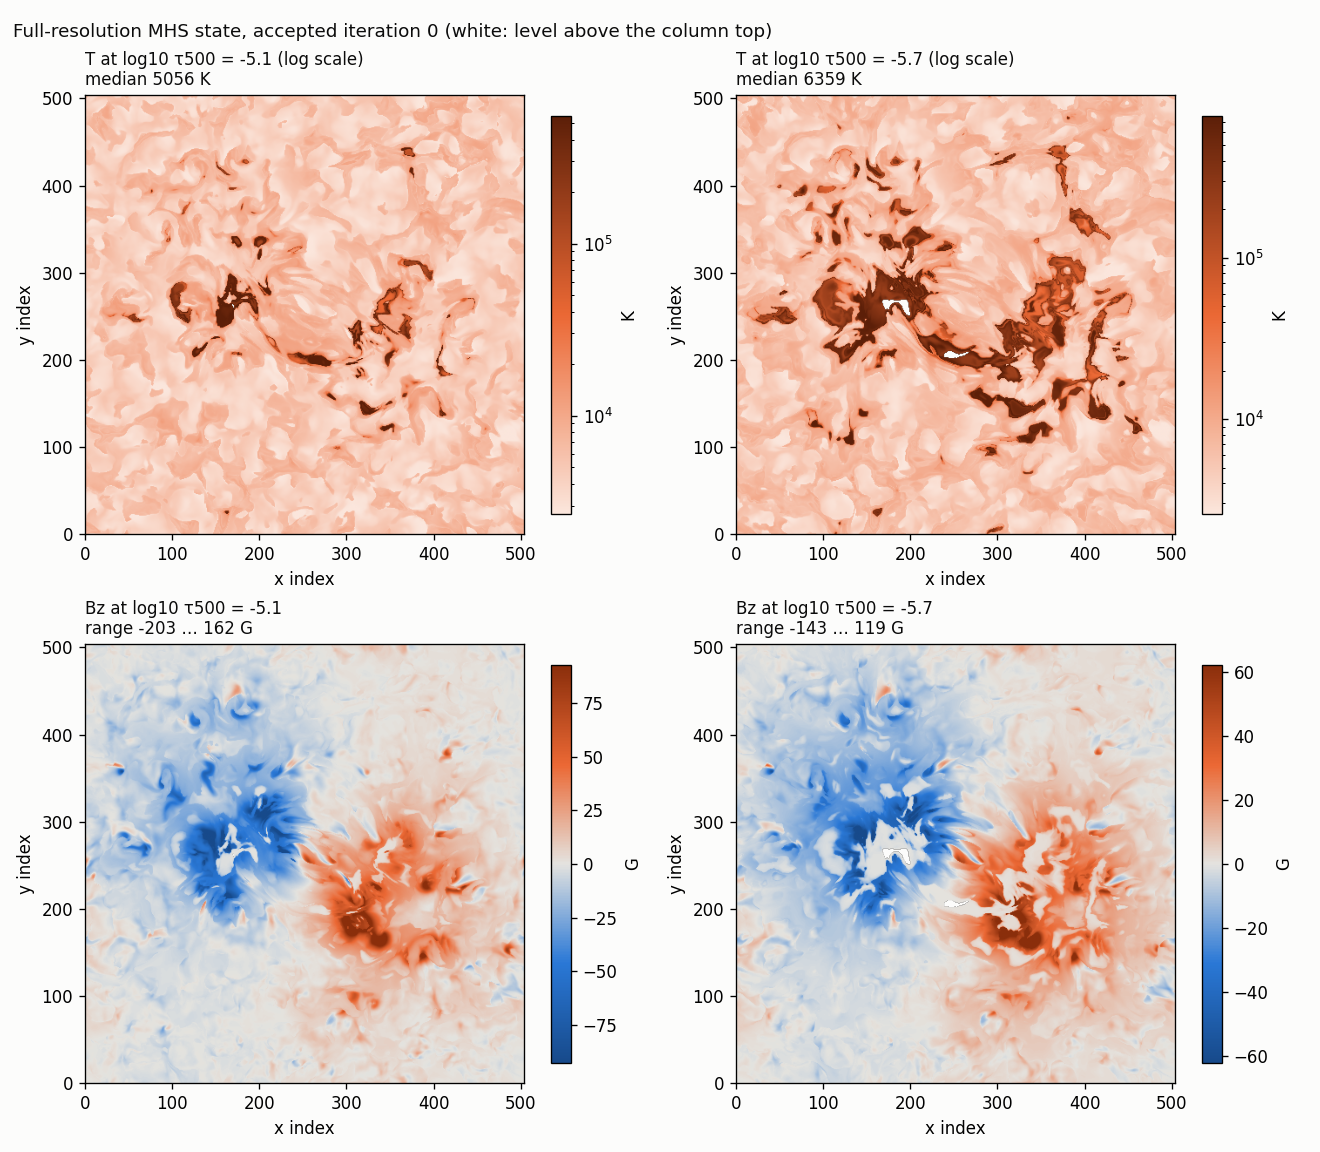
\includegraphics[width=0.83\textwidth]{figs/poisson_panel_zc1.0.png}\\[-1pt]
{\small Fig.~1. $T$ and $B_z$ on the surfaces $\log\tau_{500}=-5.1$ and $-5.7$ after the Poisson step ($z_{\rm cut}=1$\,Mm).
White: the level lies above the top of the column.}
\end{center}

\begin{center}
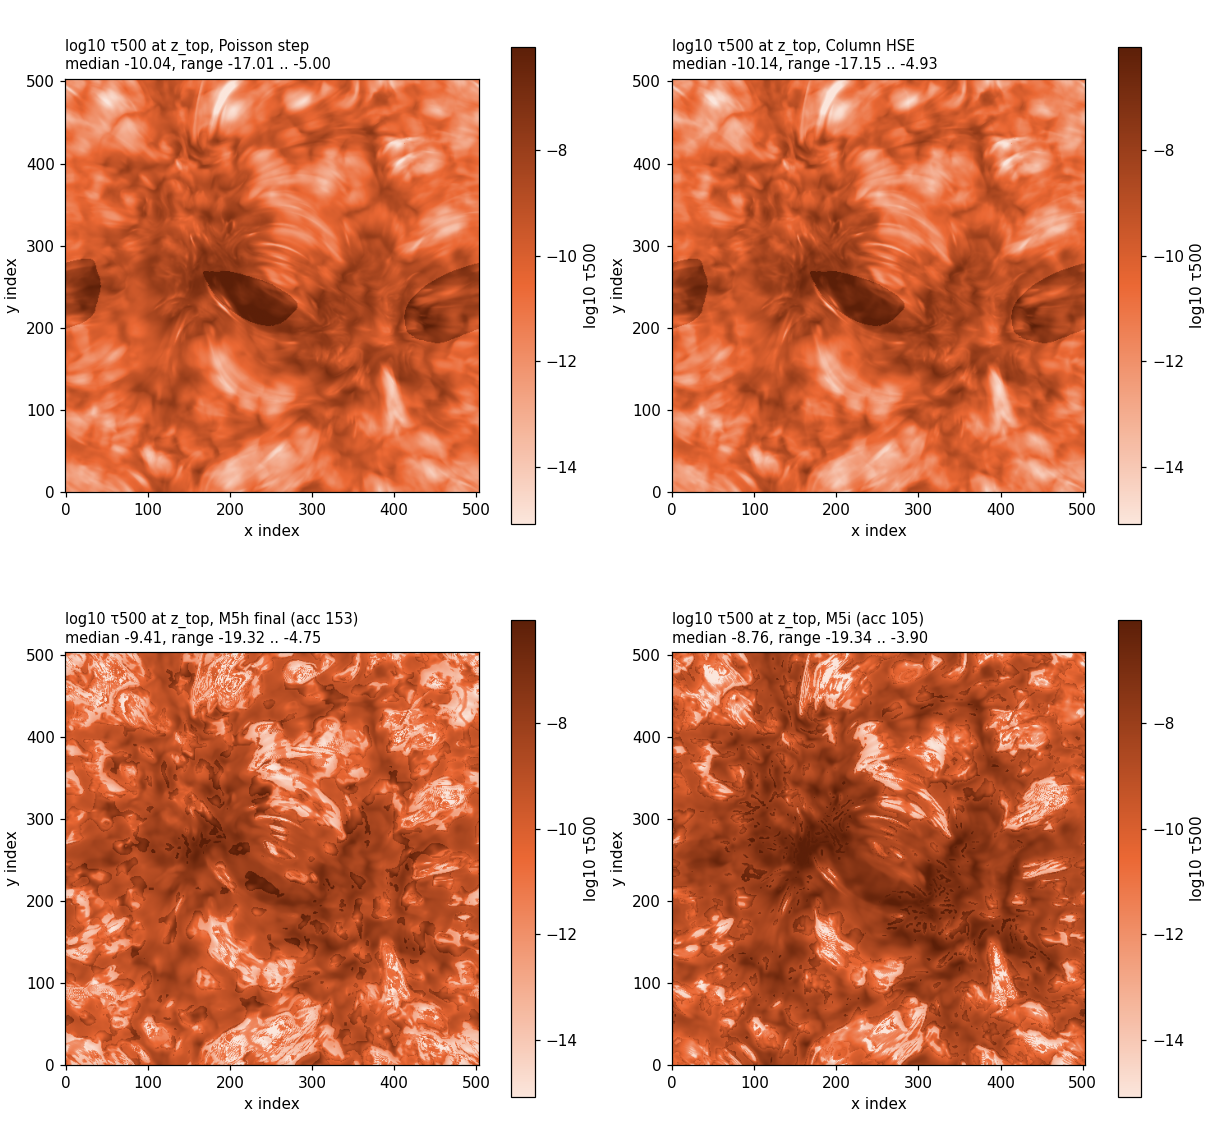
\includegraphics[width=0.83\textwidth]{figs/ztop_logtau.png}\\[-1pt]
{\small Fig.~2. $\log\tau_{500}$ at the top of the box. The Poisson step stays close to column HSE (identical above 1\,Mm by
construction); M5h and M5i, which also change the chromospheric pressure and $\B$, move the top to larger $\tau$ in patches.}
\end{center}

\section{What this means}
\begin{itemize}
\item \textbf{Speed.} Minutes instead of a day. Inside an inversion, starting from the previous iteration's pressure,
one or two Gauss--Newton steps (about 30--90\,s on the full cube) should suffice.
\item \textbf{Photosphere.} Where the lines used for inversions form ($\log\tau_{500}\gtrsim-3$, $z\lesssim0.5$\,Mm), the
step reduces the force imbalance well below that of Bifrost itself, without moving the $\tau$ scale.
\item \textbf{Chromosphere.} With $\B$ fixed, no pressure can balance a non-force-free field at low $\beta$. Above
$z_{\rm cut}$ the atmosphere is only hydrostatic. Real magnetostatic balance there needs $\B$ to change, which is what the
joint solver (M5h/M5i) does, at a much higher cost.
\item \textbf{Choice of $z_{\rm cut}$.} It is a physical parameter, not a numerical one: it marks where we stop trusting the
fixed field to be in equilibrium. A $\beta$-based cut (as FIRTEZ's \texttt{LIMIT\_MAGTERM\_BETA}) would adapt it per
column.
\end{itemize}

{\small\textbf{Technical notes.} FFTs run single-threaded because threaded FFTW crashes under Julia 1.13 (0.44\,s per
forward+inverse transform pair, so it costs little). Output file \texttt{out/poisson/poisson\_zc1.0.h5} has the layout of
an MHS checkpoint, so the same map and diagnostic scripts read it. Branch \texttt{poisson-step}, commit 08b7453.}
\end{document}
